\documentclass{standalone}

\usepackage{etoolbox}

\usepackage{tikz}
\usetikzlibrary{shapes.geometric}
\usetikzlibrary{decorations.text}
%\usetikzlibrary{knots}
\usetikzlibrary{calc}
\usetikzlibrary{math}
\usetikzlibrary{intersections}

\begin{document}
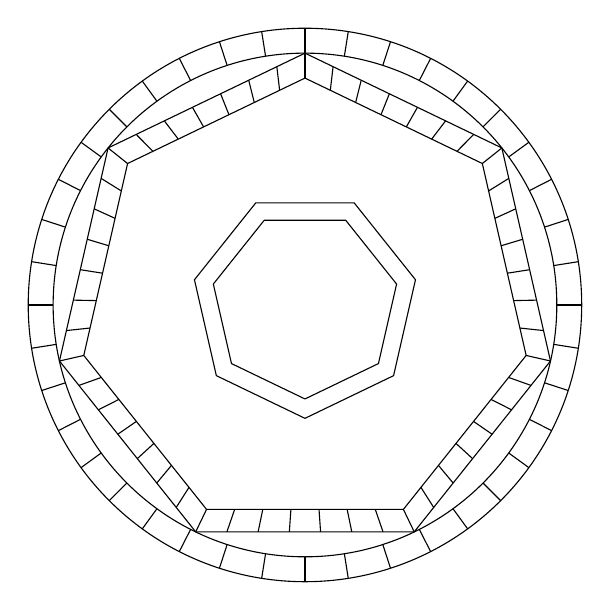
\begin{tikzpicture}
  \newdimen\rA
  \newdimen\dAB
  \newdimen\rB
  \newdimen\rC
  \newdimen\dE
  \newdimen\rD
  \newdimen\rE
  \newdimen\rF
  \newdimen\rG
  \tikzmath{
    \x = cos(180/7); % a=rx
    \rA = 100pt;
    \dAB = 9pt; % ???
    \dE = 7pt;
    \rB = \rA-\dAB;
    \rC = \rB*\x;
    \rD = (\rC*sin(180*(7-4)/(7*2))-\dE)/\x;
    \rE = \rD - 8pt;
    \rF = \rE - 7pt;
    \rG = \rF * \x;
  }


\draw circle (\rA)
      circle (\rB);
\foreach \i [evaluate={\a = \i*360/40}] in {1,...,40}
  \draw (\a:\rA) -- (\a:\rB);

\begin{scope}[regular polygon, regular polygon sides=7, line width=0pt]
  \node [minimum size=2*\rB] (eB) {};
  \node [minimum size=2*\rC] (eC) {};
  \node [minimum size=2*\rE, rotate=180] (eD) {};
  \node [minimum size=2*\rF, rotate=180] (eE) {};
\end{scope}

\draw [line join=bevel]
  \foreach \e in {eB,eC,eD,eE}
    {(\e.corner 1) \foreach \i in {2,...,7} {--(\e.corner \i)} -- cycle};

\foreach   \i [evaluate={\s = int(mod(\i,7)+1)}] in {1,...,7}
  \foreach \j [evaluate={\f = \j/7}]             in {1,...,7}
    \draw ($(eB.corner \i)!\f!(eB.corner \s)$) -- ($(eC.corner \i)!\f!(eC.corner \s)$);

%\nfoil{7}{\rC}{\dE}{*};


%\nfoil[line join=round]{5}{\rG}{2.5pt}{*};


%\node [name path=eC, draw, regular polygon, regular polygon sides=7, minimum size=2*\rC] at (0,0) {};
%\path [draw, red, dashed,regular polygon, regular polygon sides=7, minimum size=2*\rB,
%   postaction={decorate,decoration={raise=-0.5ex,text along path, text align=fit to path, text={|\fontsize{6pt}{0pt}\selectfont|SIGILLVM SANCTVM FRATERNITATIS A∴A∴}}}]
%  (64.286:34.2pt) arc (64.286:-244.286:34.2pt);


\end{tikzpicture}
\end{document}
